\subsubsection{Entity Relationship Model}\label{sec:EntityRelationModel}
The entity relationship model is a graphical representation of how database relations are structured.
This is done in an \textit{entity relationship} (ER) diagram, and is commonly used facilitate database design from specifications of enterprise schemas \cite{DBSBook}.
In the ER model, we differentiate between \textit{entity sets} representing domain elements and \textit{relationships sets} representing the connections between the domain elements. 
The entity sets are represented graphically with a rectangle and relationship sets connecting the entity sets with a diamond \cite{DBSBook}.
The attributes associated with the entity- and relationship sets can be modelled using ovals \cite{KatjaFirstPP}, however other alternatives exists.\footnote{Our style of choice is presented in Chapter 6.10 of \citetitle{DBSBook} \textit{\citefield[]{DBSBook}[]{edition}}}
Similar to the relational model, the entities (tuples) must be uniquely identified by one or more attributes. This is denoted by underlining the attributes of the entity sets. 

The ER model has notations that denote the participations each entity has in a connecting relationship \cite{DBSBook}.
In this project, we will use \text{min-max} notation; this notation denotes the minimum and maximum amount of entities participating in a relationship. 

\begin{figure}[htp]
    \centering
    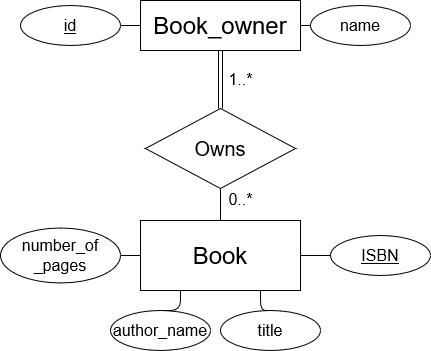
\includegraphics[scale=0.5]{Images/book_example_w_cardinality.png}
    \caption{ER diagram of the book and book owner example.}
    \label{fig:ER_Book_Example}
\end{figure}

Figure \ref{fig:ER_Book_Example} shows an ER diagram equivalent to the $book$, $owns$, and $book_owner$ relations from equation \ref{eq:bookOwnerExample} and \ref{eq:relational_schema}.
In figure \ref{fig:ER_Book_Example} we also see the participation cardinalities of the two entity sets. 
The relationship from $book\_owner$ to $owns$ is one of total participation. That is, each book owner entity must own at least one book.
\begin{figure}[h]
    \centering
    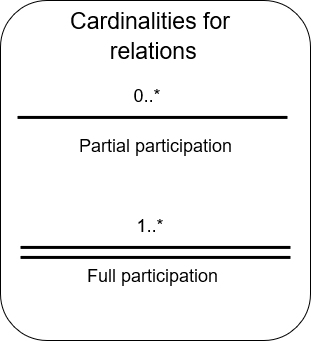
\includegraphics[scale=0.5]{Images/cardinalities.png}
    \caption{Participation ratios for ER relationships}
    \label{fig:ERDiagram_Cardinality}
\end{figure}
The participation from $book$ to $owns$ is partial. Thus the model represents that books can be in the database, even if no one owns it, that a book can be owned by multiple book owners.
Graphical notation of participation connections can be seen on figure \ref{fig:ERDiagram_Cardinality}.


Other forms of entity set exits. For instance, a weak entity set, denoted by an oval with doubled edges, is an entity set whose existence is based on another entity set. Relationship sets connecting a weak entity set to its' identifying entity set will not have any attributes\cite{DBSBook}.
A weak entity set is identified by its \textit{identifying entity set}'s primary key along with extra attributes. 
The relationship between a weak entity set and its identifying set is always many-to-one with total participation of the weak entity set.

The ER model can be converted into the \textit{relational model}. The relational model is described using relations, thus we can describe operations that can be performed on the relations using set notation and relational algebra. 
Therefore, it is useful to be able to convert an E-R model into an equivalent relational model, where domains of attributes can be well defined and operations on the entity sets described mathematically.

\subsubsection*{Converting ER Models to Relations}
When converting an ER diagram into an equivalent relational model, we must consider the domains of the attributes in the ER model, since these need to be described in the relational model. Having the domain of the relations described makes it possible to establish well-defined operations that can be performed on the relations.\\
\textbf{Strong entity sets}\\
Strong entity sets are converted by taking each attribute of the entity set, and a relation with corresponding attributes. 
The primary key of the entity set is chosen as primary key for the relation \cite{DBSBook}.\\
As an example of converting a strong entity we can use the book owner example from figure \ref{fig:ER_Book_Example}. In this example \texttt{Book} is a strong entity. The relation created from the book entity can be seen in equation \ref*{eq:StrongEntity}. The attributes from the entity are added to the relation and the primary key of the book entity, \texttt{ISBN}, is used as the primary key for the relation.

\begin{equation}\label{eq:StrongEntity}
    \begin{split}
        Book(\underline{ISBN : text} , title : text , author\_name : text , number\_of\_pages : \mathbb{Z}^+)
    \end{split}
\end{equation}
\\
\textbf{Many-to-many relationships}\\
When converting many-to-many relationships to a relation, one creates a single relation with primary key attributes from the participating entity sets \cite{DBSBook}. These keys are used as foreign key to reference the converted entities participating in the relationship. 
The remaining attributes of the entity set is similarly mapped to the relation.\\
As an example, in the book owner example there is a many-to-many relationship between a \texttt{book\_owner} and a \texttt{book} called \texttt{Owns}. As can be seen in equation \ref{eq:ManyToMany}, to convert the relationship set into a relation, the keys of the participating entities must be put into the relation. 

\begin{equation}\label{eq:ManyToMany}
    \begin{split}
        owns(\underline{owner\_id \rightarrow book\_owner}, \underline{ISBN \rightarrow book})
    \end{split}
\end{equation}
\\
\textbf{Many-to-one relationships}\\
If we have a many-to-one relationship between two sets we can combine the relationship set and the relation created from the entity set on the 'many' side into a single relation. This relation will use the primary key of the entity set as its primary key, and have a foreign referencing the relation created from the 'one' side of the relationship.\\
As an example if we for the book owner example instead assume that a book could have only one owner, it would be a many-to-one relationship. To convert the relationship set to a relation, the relationship set should be merged with the 'many' side of the relations created, which in this case would be the book as it only has one owner, but an owner can have many books. The relation created from this can be seen in \ref*{eq:ManyToOne}, which has the attributes of the initial book relation and a foreign key to the \texttt{book\_owner}.

\begin{equation}\label{eq:ManyToOne}
    \begin{split}
        Book(\underline{ISBN : text} , title : text , author\_name : text , \\number\_of\_pages : \mathbb{Z}^+, owner\_id \rightarrow Book\_owner)
    \end{split}
\end{equation}
\\
\textbf{One-to-one relationships}\\
When converting one-to-one relationships with total participation, we simply create a union of the attributes of the participating entity sets and the relationship set \cite{DBSBook}. If there is not total participation, two relations are created from the entity set, and a foreign key is placed on one of the sets.\\
As an example assume that for the book owner example that a book only has one owner, and each owner can only have one book. It would then be a one-to-one relationship. Assuming total participation between the entities, the relation can be seen in equation \ref*{eq:TotalOneToOne}, which is a union of the attributes of \texttt{book} and \texttt{book\_owner}.

\begin{equation}\label{eq:TotalOneToOne}
    \begin{split}
        owns(\underline{owner\_id \rightarrow book\_owner}, \underline{ISBN \rightarrow book}), \\
        book\_owner(name:text,\underline{owner\_id:\mathbb{Z}^+})
    \end{split}
\end{equation}


\textbf{Weak entity sets}\\
When representing weak entity sets, one creates a relation containing the attributes of the weak entity set as well as the attributes of the identifying set's primary key.
The primary key of the identifying relation will also serve as a foreign key to the identifying relation. \cite{DBSBook}.
The relationship set is simply ignored, as the relationship set will not have any attributes \cite{DBSBook}. 

% \begin{equation}\label{eq:bookOwnerExample}
%     \begin{split}
%         owns(\underline{owner\_id \rightarrow book\_owner}, \underline{ISBN \rightarrow book}), \\
%         book\_owner(name:text,\underline{owner\_id:\mathbb{Z}^+})
%     \end{split}
% \end{equation}